\documentclass[runningheads]{llncs}
\usepackage[english]{babel}
\usepackage[T1]{fontenc}
\usepackage[utf8]{inputenc}
\let\proof\relax
\let\endproof\relax
\usepackage{iftex}
\usepackage[dvipdfm]{graphicx}
\usepackage{rotating}
\usepackage{bmpsize}
\usepackage{wrapfig}
\usepackage{lscape}
\usepackage{rotating}
\usepackage{listings}
\usepackage{amsmath}
\usepackage{mathpartir} % SOS rules
\usepackage{amssymb}
\usepackage{mathtools}
\usepackage{amsfonts}
\usepackage{hyperref}
\usepackage{array}
\usepackage{booktabs}
\usepackage{multicol}
\usepackage{biblatex}
\usepackage[version=4]{mhchem}
\usepackage{siunitx}
\usepackage{longtable,tabularx}
\usepackage{times}
\usepackage{subcaption}
\usepackage{xcolor}
\usepackage{multirow}
\usepackage{enumitem}
\usepackage{calc}
\usepackage{graphicx}

\newlength{\tabwidth}
\newlength{\tabwidthi}
\newlength{\tabwidthii}
\newlength{\tabwidthiii}
\newcommand{\tabsize}{\footnotesize}
\newcommand{\thead}[1]{\tabsize\textbf{#1}}
\addbibresource{refs.bib}

\newcommand{\ie}{\emph{i.e.}}
\newcommand{\eg}{\emph{e.g.}}
\newcommand{\etc}{etc.}


\usepackage{sbnotes}
\declareauthor{sb}{Simon}
\declareauthor{sc}{Sophie}
\declareauthor{ok}{Olga}
\declareauthor{ag}{Anna}
\initcolors

\newcommand{\todomardone}[2]{\todomar{#1}{\textbf{[DONE]} #2}}
\newcommand{\todoindone}[3][]{\todoin[\textbf{[DONE]} #1]{#2}{#3}}

% Backward compatibility with notes w/o sbnotes
\newcommand{\noteok}[1]{\notemar{ok}{#1}}
\newcommand{\noteinlineok}[1]{\notein{ok}{#1}}
\newcommand{\notesc}[1]{\notemar{sc}{#1}}
\newcommand{\SC}[1]{\notein{sc}{#1}}
\newcommand{\noteinlinesc}[1]{\notein{sc}{#1}}
\newcommand{\notesb}[1]{\notemar{sb}{#1}}
\newcommand{\noteinlinesb}[1]{\notein{sb}{#1}}
\newcommand{\noteag}[1]{\notemar{ag}{#1}}
\newcommand{\noteinlineag}[1]{\notein{ag}{#1}}

% --- END COMMENTS AND NOTES -------

\definecolor{codegreen}{rgb}{0,0.6,0}
\definecolor{codegray}{rgb}{0.5,0.5,0.5}
\definecolor{codepurple}{rgb}{0.58,0,0.82}
\definecolor{backcolour}{rgb}{0.95,0.95,0.92}
\lstdefinestyle{mystyle}{
    backgroundcolor=\color{backcolour},
    commentstyle=\color{codegreen},
    keywordstyle=\color{magenta},
    numberstyle=\tiny\color{codegray},
    stringstyle=\color{codepurple},
    basicstyle=\ttfamily\footnotesize,
    breakatwhitespace=false,
    breaklines=true,
    keepspaces=true,
    numbers=left,
    numbersep=4pt,
    showspaces=false,
    showstringspaces=false,
    showtabs=false,
    tabsize=2,
    language={c++},
    % keyword highlighting
    classoffset=1, % starting new class
    alsoletter={-,>},
    morekeywords={->, SYSTEM, physical, logical, int, float, init, then, link, to, spread, collect},
    keywordstyle=\color{codepurple},
    classoffset=0
}
\lstset{style=mystyle}

\title{Definition of Chips Operational Semantics through BIP component based formalism\thanks{This work was supported by the ANR grant ANR-23-CE25-0004 (ADAPT).}}

%\author{No author given}
\author{
Anna Gallone\inst{1}\orcidID{0009-0007-3217-3896}
\and 
Simon Bliudze\inst{2}\orcidID{0000-0002-7900-5271} 
\and 
Sophie Cerf\inst{3}\orcidID{0000-0003-0122-0796} 
\and
Olga Kouchnarenko\inst{1}\orcidID{0000-0003-1482-9015}\thanks{O.~Kouchnarenko was supported by the EIPHI Graduate School (grant number ANR-17-EURE-0002).}
}
%
\institute{
Université Marie et Louis Pasteur, CNRS, UMR 6174 FEMTO-ST, F-25000 Besançon, France
\and 
Univ. Lille, Inria, CNRS, Centrale Lille, UMR 9189 CRIStAL, F-59000 Lille, France 
\and 
Univ. Grenoble Alpes, Inria, CNRS, Grenoble INP\footnote{Institute of Engineering Univ. Grenoble Alpes}, LIG, F-38000 Grenoble, France \\
\email{FirstName.LastName@femto-st.fr$^1$,FirstName.LastName@inria.fr$^{2,3}$}
}
%\def\titlerunning{Designing with Chips, Executing with BIP}
\authorrunning{A.~Gallone et al.}
\date{\today}

% Source - https://tex.stackexchange.com/a/136050
% Posted by petermeissner, modified by community. See post 'Timeline' for change history
% Retrieved 2026-05-06, License - CC BY-SA 3.0

\newenvironment{myitemize}
{ \begin{itemize}
    \setlength{\itemsep}{0pt}
    \setlength{\parskip}{0pt}
    \setlength{\parsep}{0pt}     }
{ \end{itemize}                  } 


\newcommand{\Notation}[1]{\noindent\textbf{Notation~(#1)~}}

\newcounter{defcounter}
\newcommand{\Definition}[1]{\textbf{Definition \thedefcounter~(#1)~}}

\newcommand{\eqdef}{\stackrel{\mathclap{\normalfont\mbox{\footnotesize def}}}{=}}
\newcommand{\aoverb}[2]{\stackrel{\mathclap{\footnotesize #1}}{#2}}
\newcommand{\s}{\hspace{1em}}
\newcommand{\halfs}{\hspace{0.5em}}
\newcommand{\mprod}{\text{ \textbf{m} }}
% Source - https://tex.stackexchange.com/a/371469
% Posted by Moriambar, modified by community. See post 'Timeline' for change history
% Retrieved 2026-05-29, License - CC BY-SA 4.0
\newcommand{\myrule}{\par\noindent\rule[-1pt]{0.5\textwidth}{0.4pt}\\}

\newcommand{\F}{\mathbb{F}}

\begin{document}

\maketitle

\begin{abstract}
    This Document contains a draft of the definition of operational semantics for Chips through the lens of the BIP Framework (which has been proven to be correct by construction).

    \keywords{First keyword  \and Second keyword \and Another keyword.}
\end{abstract}

\section{Introduction}
Chips is a language for designing complex systems models based on the formalism of functional block diagrams. It also features programming primitives for the specification of the coordination mechanisms one would want to implement in systems comprising large sets of components. Our primary intention with this language was to compile it into models within the BIP framework. To build a robust and provable compilation pipeline from Chips to BIP, we used Model Driven Engineering technics that are implemented within the Eclipse Modeling Framework. Our compilation process, described in Figure~\ref{fig:EMFpipeline}, is based on a metamodel of the Chips language (\texttt{chips1.1.ecore}) that allow us to use any serialized Chips model as a source artifact to generate a BIP compatible target model artifact. Such BIP models are then inserted in the BIP compiler middle-end part to be directly reused as if the compiler just parsed a BIP program. Such pipeline benefits the insurances provided by the Chips and BIP models automatic validation relatively to their languages Meta-models and also avoids the introduction of bugs during a potential code generation step. Hereafter, we describe formally the principles on which the meta-models used are grounded and give arguments on what exactly are the transformations that allow to build a BIP model from a Chips specification. 
As the BIP operational semantics is fully defined, and its compilation process proven to be correct, these elements together provide an interpretation of the Chips operational semantics under the lense of the subset of the BIP framework our transformation rules define. The following Section~\ref{sec:ChipsMM} proposes a definition of the Chips Models elements based on its metamodel, then Section~\ref{sec:BipMM} recalls the main elements of the BIP models that we use during the transformations that we formally present in Section~\ref{sec:Chips2Bip}.


\begin{figure}
    \centering
    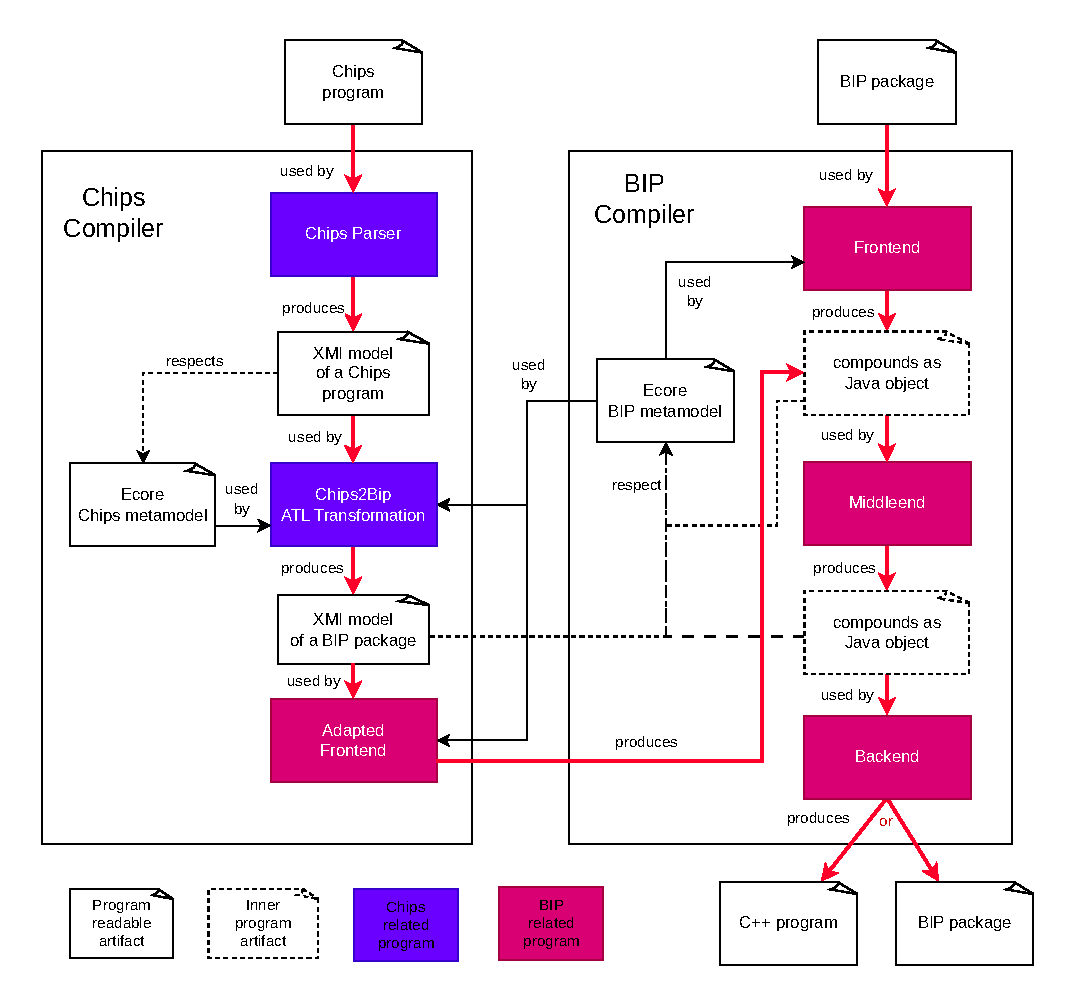
\includegraphics[width=0.8\columnwidth]{./imgs/EMFpipeline.pdf}
    \caption{Eclipse Based Model Transformation Pipeline}\label{fig:EMFpipeline}
\end{figure}

\section{Definition of the Chips models architecture}
\label{sec:ChipsMM}

Though it is based on functional block diagrams, in the graph that functions form, our Chips language doesn't rely solely on a function-output-to-function-input type of edges between the different vertices. Indeed, Chips models also care about concepts like distribution of dataflows among sets of devices and embedding relationships between software and hardware. These three concepts together form what Chips models try to capture. To describe a Chips model $M$, we therefore consider a tuple of three graphs $M \eqdef (G_N,G_F,L)$ where:
\begin{itemize}
    \item $G_N$ is the network graph, representing which component can directly transmit information to another,
    \item $G_F$ is the functional graph, representing the dataflows between the functions of the system, and
    \item $L$ is the linking forest, a set of trees that associate functions to the nodes of the networks designed.
\end{itemize}

Following subsections give a formal definition of each one of these graphs and their compounds. 
But beforehand, it is necessary to mention what actually are types, values and variables manipulated by the the model components we are about to define. To do so, we will assume the existence of an infinite set $\Sigma$ containing labels from which to draw names for our elements. 

\begin{definition}\label{def:ChipsPrimitiveType}
    A \emph{Chips Primitive Type} is either $int$ (the set of binary representable relative integers), $float$ (the set of binary representable floating point values) and $bool$ (the set of $\top$ and $\bot$), or fixed multidimensional arrays of any one of the mentioned type.
    An element of any of this type is what we will call a ``data''. The set of these types will be refered to as $\mathbb{T}$.
\end{definition}

\begin{definition}\label{def:ChipsPrimitiveType}
    A \emph{Primitive value} is a couple $(data, stop) \in \mathbb{T} \times bool$. In such definition, $d$ is the data held by the chips value and $stop$ is an artifact of simulation that signifies the value hasn't been updated recently (in the sense of synchronous languages clocks). In this paper, we call the set of Chips primitive values $\mathbb{X}$. 
\end{definition}

\paragraph{Notation} In the rest of this document, we will refer to elements mentioned during the definiton of any abstract object with a dot notation. For instance, to refer to the data held by a given $v \in \mathbb{X}$, we write $v.data$.

\begin{definition}\label{def:PrimitiveVariable}
    A \emph{Primitive variable} is a couple $(id,type) \in \Sigma \times \mathbb{T}$. $id$ is the name uniquely identifying each primitive variables and $type$, as expected, is the type of the primitive variable. Along with each variable, we assume the existence of a function $value: \Sigma \times \Sigma \mapsto \mathbb{X}$ which, for each primitive variable and according to the id of the element containing it, returns the current value of the variable. Such valuation may change if the variable is affected a new value.
\end{definition}

\subsection{Network Graphs}
\label{sec:networkgraphs}

Let us define define the primitive model elements that constitute the vertices of Chips network graphs (\emph{nodes}) and their specific kind of attribute (\emph{channels}).

\begin{definition}\label{def:Channel}
    A \emph{Channel} is a couple $(id,cht) \in \Sigma \times \Sigma$. $id$ is a name uniquely identifying each channel and $cht$ is another name that allows to distinguish the different sorts of channels defined by the user. Such concept serves to model the connectivity features of an element of a model.
\end{definition}

\begin{definition}\label{def:Node}
    The types and names of a node's attributes are defined by that node's type. A \emph{node type} is a couple $nt = (CH, CTX)$ where:
    \begin{itemize}
        \item $CH$ is a set of channels.
        \item $CTX$, which we call \emph{contextuals} in the Chips language, is a set of primitive variables that are read and write accessible by processes\footnote{Such processes are explained in Definition~\ref{def:FunctionalBlock}.} located in the node.
    \end{itemize}
    We call the set of defined node types $\mathbb{T}_{node}$.
    A \emph{node instance} is a couple $n=(nt,id)$ where:
    \begin{itemize}
        \item $nt \in \mathbb{T}_{node}$ and
        \item $id\in\Sigma$ uniquely identifies this instance.
    \end{itemize}
\end{definition}


\begin{definition}\label{def:NetworkGraph}
    A \emph{Network Graph} is a couple $G_N = (N,C)$ where:
    \begin{itemize}
        \item $N$ is a set of nodes instances.
        \item $C \subset \{(n,ch, n', ch') \text{ | } n,n' \in N, ch \in n.nt.CH, ch' \in n'.nt.CH \text{ and } ch.cht = ch'.cht \}$ is a set of connections inbetween nodes. $(n,ch)$ is the source of the connection and $(n',ch')$ is the sink of the connection.
        \item No channel can be a source or sink more than once. \\Formally $\forall c_1,c_2 \in C, c_1.ch \neq c_2.ch \wedge c_1.ch' \neq c_2.ch'$.
    \end{itemize}
\end{definition}

This definition of networks lets us draw a minimal representation of any kind of interacting entities. The fact that channels are typed allows some robustness and modularity in the design of our components : A declared USB port cannot communicate with a WIFI card for instance.

\begin{remark}\label{rem:PhysicalVirtualDistinction}
    Chips syntax makes a differentiation of network nodes in two categories, physical and virtual nodes (respectively called \emph{physical} and simply \emph{object}). It serves the purpose of checking the feasibility of embedding relationship, with in mind, the goal of generating code for real systems. Therefore, it doesn't impact the Chips semantics, we will not cover here the elements of Chips language relative to the distinction between physical and virtual nodes.
\end{remark}

\subsection{Functional Graphs}
\label{sec:functionalgraphs}

To build the definition of a functional graph, we first need to introduce what forms their vertices. Such elements are embodied by functional blocks.

\begin{definition}\label{def:FunctionalBlock}
    Let $G_N$ be a network graph. A correctly defined Chips \emph{functional block type} is a tuple $(I, O, CTX, S, f)$, where:
    \begin{itemize}
        \item $I$ and $O$ are finite disjoint sets of respectively input and output primitive variables,
        \item $CTX \subseteq \cup_{n \in G_N.N} n.nt.CTX$ is the set of contextual primitive variables read and write accessed by the functional block.
        \item $S$ is a finite set of state primitive variables.
        \item $f$ is a function of $\mathbb{X}^{I \cup CTX \cup S} \mapsto \mathbb{X}^{O \cup CTX \cup S}$.
    \end{itemize}
    And a \emph{functional block instance} is a couple $(fbt, id)$ where:
    \begin{itemize}
        \item $fbt$ is the functional block type of the instance and
        \item $id\in\Sigma$ uniquely identifies each instance of functional block. 
    \end{itemize}
    We call the set of all instances of functional blocks $\F$.
\end{definition}

Now that we have defined the vertices for our functional graphs and what data they treat, we need to define our edges. Chips allows to design two different kinds of edges for their functional graphs, regular source-to-sink relationship (simple dataflow) and one-source-to-many-sinks or many-sources-to-one-sink relationship (collective dataflow).

\begin{definition}\label{def:SimplDataflow}
    Let $f,f' \in \F$ . If $f.O$ and $f'.I$ are both non-empty sets, then a \emph{simple dataflow} can be defined as $(source,sink) \in f.O \times f'.I$.
\end{definition}

Simple dataflows allow to specify one-to-one relations. With this structure, if need be to define a broadcast or aggregation behavior while acknowledging the topology of a network, a significant description overhead has to be faced. For instance, let us draw a network of four devices \textbf{A}, \textbf{B}, \textbf{C} and \textbf{D}, where information can only flow between the pairs (\textbf{A},\textbf{B}), (\textbf{B},\textbf{C}) and (\textbf{C}, \textbf{D}) as shown by figure~\ref{fig:smallnet}. If \textbf{A} needs to broadcast information to \textbf{B}, \textbf{C} and \textbf{D}, the situation changes drastically whether or not we decide to take account of the network topology. If we do, each involved component would require new dataflows for re-transmitting any information that is not addressed to it. On a small example like this one, it may not look like much, but for any chain of $n$ components, instead of defining one dataflow from the source of the broadcast to each one of the $n$ target functional blocks, this represents the definition of $\Sigma_{i=0}^{n}i$ distinct dataflows, which in terms, can be reduced to a spatial complexity of $O(n^2)$.

\begin{figure}
    \centering
    \includegraphics[width=\columnwidth]{./imgs/DataflowOverHead.pdf}
    \caption{Model architecture allowing a broadcast operation among a chain of four functional blocks using simple dataflows}\label{fig:smallnet}
\end{figure}

Moreover, it becomes very hard to design the right definitions for our functional blocks inputs and outputs if we want to simulate broadcast or aggregation operations enchanced with on-the-fly computations, or even if our topology isn't a chain, but a more complex structure. This is why we also need to design other kinds of dataflows, which we call \emph{collective dataflows}.

\begin{definition}\label{def:CollectiveDataflows}
    For a given network graph $G_N$ making use of at least one node type $nt$, a \emph{collective dataflow type} is defined in the form of a quadruple $\left(t \times ACC \times nt \times cf\right)$ where:
    \begin{itemize}
        \item $t \in \{spread, collect\}$,
        \item $ACC \in \mathbb{X}^n$ with $n\in\mathbb{N}$,
        \item $nt \in \mathbb{T}_{node}$
        \item $cf : \mathbb{X}^{ACC} \times \mathbb{X}^{nt.CTX} \mapsto \mathbb{X}^{ACC\times nt.CH}\times \mathbb{X}$, is a function mapping the valuation of an accumulator and contextual primitive variables of the support node onto the co-domain composed of one accumulator per channel of the support node and one value being the input of a functional block.
    \end{itemize}
    We call the set of collective dataflow types $\mathbb{T}_{collective}$.
    Let $f,f' \in \F$ . If $f.O$ and $f'.I$ are both non-empty sets. Then an instance of a collective dataflow is defined as:\\
    $(source, dft, sink) \in f.O \times \mathbb{T}_{collective} \times f'.I$
\end{definition}

This way, a functional graph can be synthesized without worrying about the supporting network underneath. As long as the one-to-one relations between each node are specified, this last definition allows to distinguish propagation or aggregation for any possible path for the information across the network. Which leads us now to the definition:

\begin{definition}\label{def:FunctionalGraph}
    Chips models draw \emph{functional graphs} in the form of $G_F = (F, DF\cup CDF)$ where:
    \begin{itemize}
        \item $F \subset \F$ is the set of instantiated functional blocks in a model,
        \item $DF \cup CDF$ is the set of declared simple and collective dataflows defined over $G_F$,
        \item each functional block input (respectively output) is the sink (resp. source) of at most one simple dataflow,
        \item each functional block input is the sink of at most one collective dataflow of type $spread$,
        \item each functional block output is the source of at most one collective dataflow of type $collect$,
        \item each functional block input (resp. output) is the sink (resp. source) of at least one dataflow (simple or collective).
    \end{itemize}
\end{definition}

\subsection{Linking Forests}
\label{sec:linkingforests}

Since both collective connectors and functional blocks definitions (elements of $G_F$) are based upon informations of nodes (elements of $G_N$), we still need to define the glue that maps $G_F$ onto $G_N$.

\begin{definition}\label{def:LinkingForest}
    Let $G_N$ be a network graph and $G_F$ be a functional graph for which every collective dataflow instance relies on node types used in $G_N$.
    A \emph{linking forest} $L$ is a set of directed rooted trees that have leaf vertices being elements of $G_F.F$ (i.e. functional blocks) and other vertices being elements of $G_N.N$ (i.e. nodes). Edges are oriented toward the root of the tree they belong to.
\end{definition}

\paragraph{Notation} For any node $n$ belonging to a tree of a liniking forest $L$, any element $x$ of any subtrees of $n$ is said to be \emph{embedded} in $n$. In such case, we write $x \sqsubset_L n$.

\paragraph This definition lets us also define what is a well formed linking forest over $G_N$ and $G_F$. This concept depends on how contextual primitive variables defined in elements of $G_N.N$ are manipulated by elements of $G_F.F$. The related elements in $G_F$ are those of $G_F.F$ and $G_F.CDF$.

\begin{definition}\label{def:FContextualsAccessibility}
    Let $G_N$ be a network graph. Let $G_F$ be a functional graph defined over $G_N$ for which every type of $G_F.CDF$ relies on types of nodes of $G_N$. Finally, let $L$ be a linking forest over elements of $G_N$ and $G_F$. The \emph{contextual accessibility} is a relation between contextuals mentioned in $G_F$ and those defined in $G_N$ :
    \begin{multline*}
        \forall f \in G_F.F, \forall c \in f.CTX, \forall n \in G_N.N,\\ c \in n.nt.CTX \text{\hspace{2em}}\wedge\text{\hspace{2em}} f \sqsubset_L n \\
        \wedge (\forall n' \in G_N.N, c \in n'.nt.CTX, f \sqsubset_L n' \sqsubset_L n \Rightarrow n = n')\\
        \Rightarrow value(c, n) = value(c, f)
    \end{multline*}
\end{definition}

\begin{definition}\label{def:CDFContextualsAccessibility}
    The $(source, dft, sink)$ representation is a shorthand for representing a \emph{set} of collective dataflows.\\Let $G_N$ a network graph, let $n,n' \in G_N.N$ such that $n.nt = n'.nt$ (which we will simply call $nt$ here) and there exists a single path in $G_N$ going from $n$ to $n'$ only using nodes of type $nt$.\\Let $G_F$ a functional graph over $G_F$. Let $f,f' \in G_F.F$ and let $L$ a linking forest such that $f\sqsubset_L n$ and $f'\sqsubset_L n'$.\\If there exists $cdf = (source, dft, sink) \in D_F.CDF$ with $source \in f.O$, $sink \in f'.I$ and $dft.nt = nt$, then we instanciate one of the above mentionned collective dataflow per node on that path. 
    The result of the propagation or aggregation of data from $f$ to $f'$ is computed by the reccursive composition of the consecutive $cdf.cf$ along the path from $n$ to $n'$. The accumulator that serves as input for the next call of $cdf.cf$ depends on the channel used to create the path. The contextual primitive variables values used by each function call are the ones that can be retrieved by the $value$ function in the scope of each node instance on the path. \noteag{Really not sure about that definition. I'm pretty sure I'll need a diagram.}
\end{definition}

The conjunction of network graphs, functional graphs and linking forests correspond to the complete set of concepts that Chips intends to work with. It features the possibility to design both topological and business aspects of a cyber-physical system and lets the designer take into account any of the two aspect to base the implementation of the other one.

\section{(Partial) Definition of the BIP component model}
\label{sec:BipMM}

BIP is a component based framework that lets one design a wide range of systems in a discrete way, i.e. in the form of synchronized automata and or petri networks. It is a mature framework that lead to the redaction of many papers, among which its formal operational semantics can be found. This section recalls the concepts of the BIP framework that are used during the compilation of Chips models into BIP ones.


\section{Transformation rules of Chips Models into BIP components}
\label{sec:Chips2Bip}

To generate a Chips model within the BIP framework, we deigned a specific type of compound that we can derive to build any kind of functional block. Then our transformation method uses synchronous connectors inbetween instances of compounds.
In this section, we will describe what such compounds are made of according to the nature of their inputs/outputs. Then, we will dive into the way we organize the architecture of our models based on the topology defined by network graphs.

\paragraph{Notation}\label{not:TransformationRule}
To describe our transformation rules, we use statements in the following form:
\[
\cfrac{P_0 \dots P_n}{X \Rightarrow Y}~label
\]
Where:
\begin{itemize}
    \item $X$ is a set of elements pre-existing to the application of the transformation rule,
    \item $Y$ is a set of elements produced by the application of the rule
    \item $P_0 \dots P_n$ is a set of premisses of the transformation rule,
    \item $label$ is the name of the rule.
\end{itemize}
Ususally, elements relative to the Chips models will be written in first position (instead of $X$) and elements relative to the BIP models in second position (instead of $Y$).

\begin{definition}\label{def:PortModel}
    We use, in the context of this paper, the concept of \emph{valued ports} instead of simple \emph{ports}. A \emph{valued port} is a tuple $p = (id,vars) \in  \Sigma \times 2^\Sigma$ where:
    \begin{itemize}
        \item $id$ is a uniquely identifying label, and 
        \item $vars$ the set of the identifiers of a finite number of primitive variables that have already been defined.
    \end{itemize}
    Valued ports can act as interfaces between components, both in term of synchronization and in term of data exchange. A port $p$ for which $p.vars = \emptyset$ can only serve synchronization purposes. For a given finite set of primitive variables $V$, we also define $\mathbb{P}_V \subset \Sigma \times \Sigma^V$, the set of all possible ports that contain identifiers of elements of $V$. When defining a port $p$ over $n\in\mathbb{N}$ anonymous variables, through misuse of language, we write that $p \in \mathbb{P}_n$. We refer to the $i$-th variable held by such $p$ with the notation $p[i-1]$, assuming there exists a total order over the elements of $\Sigma$ so there is no ambiguity on what variable has index $i$.
\end{definition}

\begin{definition}\label{def:InteractionModel}
    For a set of ports $P$, an \emph{interaction} is a couple $i = (a, update)$ where:
    \begin{itemize}
        \item $a$ is a non-empty subset $a \subseteq P$ of ports and
        \item $update:2^\mathbb{X} \mapsto 2^\mathbb{X}$ is a endomorphism over the set of variables defined in the same scope.
    \end{itemize}
\end{definition}

\begin{definition}\label{def:BehaviorModel}
    To describe the behavior of a BIP atomic component, we will use an Augmented-\emph{Labelled Transition Systems} (LTS) defined in the form of a tuple $B = (Q,P,X,\rightarrow, q_0)$ where $Q$ is a set of \emph{states}, $P$ is a set of \emph{valued ports}, $X$ is a set of primitive \emph{inner variables} and $q_0$ is the initial state. Finally, using $G$ as the set of boolean expressions over $X$, $\rightarrow \subseteq Q \times 2^P \times Q \times G$ is a set of \emph{transitions}, each labelled by an interaction over $X$. A transition is enabled if its last component evaluates to $\top$.
\end{definition}

\paragraph{Notation} We will use the notation $a\xrightarrow{p}b$ to simplify the definition of a transition $(a, \{p\}, b, \top)$.

\subsection{Base functional transformations}
We describe here how to generate, from our previous Chips models, the required BIP components to assemble to realize an architecture able to simulate operations of classical synchronous languages. Namely, we show how to construct BIP entities that read any number of input signals, produce any number of output signals, and act altogether according to a set of constraints that emulate a clock tick. Since each signal must come from a designed Chips functional block, our first transformations focus on this type of element.\\
\begin{wrapfigure}[13]{r}{0.6\columnwidth}
    \centering
    \vspace{-6ex}
    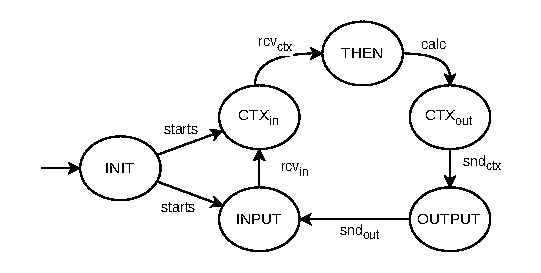
\includegraphics[width=0.65\columnwidth]{imgs/core.pdf}
    \caption{The atomic \emph{core} FSM template used for every Chips functional block definition}\label{fig:core}
\end{wrapfigure}
For the business part, each functional block definition is translated as a six states Augmented-LTS (which we will call the \emph{core} FSM) as described in Figure~\ref{fig:core}. 
In such FSM, $INIT$ is our initial state, no final state exists because our system is suppose to run until a deadlock is reached and once the business process has started, our components realizes its operations over and over.
\\
Formally, our first transformation rule is about turning a Chips functional block type into such core FSM :
\[
\inferrule
{
    starts, calc \in \mathbb{P}_\emptyset
    \\
    rcv_{ctx}, snd_{ctx} \in \mathbb{P}_{CTX}
    \\
    rcv_{in} \in \mathbb{P}_I
    \\
    snd_{out} \in \mathbb{P}_O
    \\
    Q = \{INIT, THEN, INPUT, OUTPUT, CTX_{in}, CTX_{out}\}
    \\
    P = \{starts,rcv_{in},rcv_{ctx},calc,snd_{ctx},snd_{out} \}
    \\
    X = I\cup O\cup CTX\cup S
    \\
    starting \in \{\top,\bot\}
    \\
    i_0=(INIT, \{starts\}, INPUT, starting)
    \\
    i_1=(INIT, \{starts\}, CTX_{in}, \neg starting)
    \\
    r_0= INPUT\xrightarrow{rcv_{in}} CTX_{in}
    \\
    r_1= CTX_{in}\xrightarrow{rcv_{ctx}}THEN
    \\
    t=THEN\xrightarrow{calc}CTX_{out}
    \\
    s_0=CTX_{out}\xrightarrow{snd_{ctx}}OUTPUT
    \\
    s_1=OUTPUT\xrightarrow{snd_{out}}INPUT
    \\
    \rightarrow = \{i_0,i_1,r_0,r_1,t,s_0,s_1\}
}
{(I,O,CTX,S,f) \Rightarrow (Q,P,X,\rightarrow, INIT)}~core
\]
\begin{remark}\label{rem:DefaultStart}
    In the $core$ transformation rule, we purposly omit to define how to choose the correct truth value for the $starting$ variable. We assume such values will always (if possible) be chosen so the whole system doesn't start in a deadlock state.
\end{remark}

For a given Chips functional block type, the interaction associated to each transition is defined by Table~\ref{tab:CoreInteractions}\footnote{Evaluations vary according to the functional block instance, the other instances communicating with it an the nodes to which it is linked to.}.

\begin{table}
    \centering
    \begin{tabular}{|c|c|c|}
        \hline
        ~port involved~ &~updated variables~& new value(s)\\
        \hline
        $starts$    & $S \cup I$            &~ evaluation of the \texttt{init} section and input default values~\\
        $rcv_{in}$  & $I$                   & values received via input port \\
        $rcv_{ctx}$ & $CTX$                 & evaluation of linked contextual values \\
        $calc$      & $S\cup O \cup CTX$    & evaluation of $f$ with parameters being values of $I \cup S \cup CTX$ \\
        $snd_{ctx}$ & $\emptyset $          & (no update)\\
        $snd_{out}$ & $\emptyset $          & (no update)\\
        \hline
    \end{tabular}
    \caption{Definition of the $update$ function of interactions for a core FSM of a given functional block type $(I,O,CTX,S,f)$}\label{tab:CoreInteractions}
\end{table}

The second transformation step to achieve is the set of auxiliary FSMs that allow the reception (respectively emission) of each input value (resp. output value) in whatever order. To do so, Let us introduce the $buffer$ rule:
\[
\inferrule
{
    var \in \Sigma \times \mathbb{T}
    \\
    Q = \{RCV,SND\}
    \\
    d \in \mathbb{X}
    \\
    P = \{r,s\} \subset \mathbb{P}_{\{d\}}
    \\
    \rightarrow = \{RCV\xrightarrow{r}SND,SND\xrightarrow{s}RCV\}
    \\
    B = (Q,P, \{d\},\rightarrow,RCV)
}
{var \Rightarrow B}~buffer
\]
The principle behind the definition of input buffer components is to store temporarily each value sent to our $core$ FSM. When the $core$ FSM reaches its $INPUT$ state, it is ready to simultaneously free each one of its input buffer as it consumes their values. A reciprocal mechanism is applied for the output buffer components. To obtain such behavior, the interactions of buffers are defined according to Table~\ref{tab:BufferInteractions}\footnote{Same remark as for the previous table.}.

\begin{table}
    \centering
    \begin{tabular}{|c|c|c|}
        \hline
        ~port involved~ &~updated variables~&~new value~\\
        \hline
        $r$ & $d$           & $\text{~if~} r[0].stop \text{~then~} (d.data, \top) \text{ else } (r[0].data, \bot) \text{~}$\\
        $s$ & $\emptyset $  & (no update)\\
        \hline
    \end{tabular}
    \caption{Definition of the $update$ function of interactions for a buffer FSM $(Q, \{r,s\}, \{d\},\rightarrow,RCV)$}\label{tab:BufferInteractions}
\end{table}

To conclude the construction of a functional block, we need to define the way values are transmitted from the input buffers to the core component, and then to the output buffers. We do so by using BIP interactions between ports. More specifically, our transformations never makes use of BIP trigger port interactions, so our definition of what look like can be simplified as follow:
\begin{definition}\label{def:DataflowInteraction}
    Let $n\in \mathbb{N}$, Let $s,r \in \mathbb{P}_n$ be two ports provided by two different BIP components. A \emph{dataflow} is a BIP rendez-vous interaction between $s$ and $r$ in which the values stored in $s.vars$ are set as the values stored in $r.vars$, with respect to their order of identifiers.\\
    We write such interaction $s\curvearrowright r$.
\end{definition}

One one hand, our $\#I$ input buffers and $\#O$ output buffers are components with ports of arity one. On the other hand, our \emph{core} atoms feature $rcv_{in}$ and $snd_{out}$ ports that expose respectively $\#I$ and $\#O$ values. To allow the correct transmission of data at the input and output interfaces of our functional block type, let us introduce a variation of the dataflow interaction:

\begin{definition}\label{def:SplitDataflow}
    Let $n\in \mathbb{N}$, let $(s_i)_{i\in [0,n)} \in (\mathbb{P}_1)^n$ be a set of ports and $ r\in \mathbb{P}_n$ a port, each provided by a different BIP component. A \emph{split dataflow} is a BIP rendez-vous interaction between $(s_i)_{i\in [0,n)}$ and $r$ where the value of the $s_i$ port's variable is affected to the $i$-th variable of the $r$ port (according to the order of $r$'s variable identifiers).\\
    Symetrically, let $n\in \mathbb{N}$, let $ s\in \mathbb{P}_n$ be a port and $(r_i)_{i\in [0,n)} \in (\mathbb{P}_1)^n$ be a set of ports each provided by a different BIP component. A \emph{merge dataflow} is a BIP rendez-vous interaction between $s$ and $(r_i)_{i\in [0,n)}$ where the value of the $i$-th variable of the $s$ port (according to the order of $s$'s variable identifiers) is affected to the $r_i$ port's variable.\\
    We respectively write these two operations $\{s_i \text{~|~} i\in [0,n)\} \curvearrowright r$ and $s \curvearrowright \{r_i \text{~|~} i\in [0,n)\}$.
\end{definition}

We can now compose the transformation rules that turns our Chips functional blocks into a complete definition of usable BIP compound. The following transformation can be summed up as the addition of the merge interaction to provide the values to the core component and the split interaction to provide computed values to the output buffers:
\[
\inferrule
{
    \forall io \in I\cup O
    \\
    \inferrule
    {
        \ldots
    }{
        io \Rightarrow B_{io}
    }~buffer
    \\
    \inferrule
    {
        \ldots
        \\
        P = \{\ldots, rcv_{in}, snd_{out}, \ldots\}
        \\
        \ldots
    }{
        (I,O,CTX,S,f) \Rightarrow (Q,P,X,\rightarrow, INIT)
    }~core
    \\
    \{B_i.P.s \text{~|~} i\in I\} \curvearrowright rcv_{in}
    \\
    snd_{out} \curvearrowright \{B_o.P.r \text{~|~} o\in O\}
}
{
    (I,O,CTX,S,f)\Rightarrow \{B_k \text{~|~} k\in I\cup O\} \cup \{(Q,P,X,\rightarrow, INIT)\}
}~compound
\]

\begin{remark}\label{rem:NoCTX}
    One can notice the interactions do not account for the ports dedicated to contextual primitive variables. The reason is that we haven't defined how nodes are materialized yet. Definitions of the network topology and its elements are left for section~\ref{sec:TopologyBasedOperations}. 
\end{remark}

Now that we have completed the definition of the transformation rules relative to the generation of one functional block BIP representation, we can focus on \emph{sets} of such components. Then, further transformations treat the case of whole Functional Graphs.

\[
\inferrule
{
    \forall fb \in F
    \\
    \inferrule{
        \ldots
    }
    {
        fb.fbt \Rightarrow COMP_{fb}
    }~compound_{fb}
}
{
    (F,DF\cup CDF)\Rightarrow \{COMP_{fb} | fb \in F\}
}~compounds
\]

\[
\inferrule
{
    \forall df \in DF,\exists (f_s, f_r) \in F^2,\exists (k_s, k_r) \in f_s.O \times f_r.I, df.source = k_s, df.sink = k_r
    \\
    \inferrule{
        \ldots
    }
    {
        k_s \Rightarrow B_{s}
    }~buffer_s
    \\
    \inferrule{
        \ldots
    }
    {
        k_r \Rightarrow B_{r}
    }~buffer_r
    \\
    B_{s}.P.s \curvearrowright B_{r}.P.r
}
{
    (F,DF\cup CDF)\Rightarrow \{B_s, B_r\}
}~simpledf
\]

The rules $compounds$ and $simpledf$ constitute the strict necessary to compose systems where no operation relies on a network graph.

\subsection{Topology based transformations}
\label{sec:TopologyBasedOperations}



\printbibliography

\end{document}